\documentclass[sigconf]{acmart}

\usepackage{booktabs} % For formal tables

\usepackage{graphicx}
% Used for displaying a sample figure. If possible, figure files should
% be included in EPS format.
%
% If you use the hyperref package, please uncomment the following line
% to display URLs in blue roman font according to Springer's eBook style:
% \renewcommand\UrlFont{\color{blue}\rmfamily}

\usepackage{siunitx}

\usepackage{tikz}
\usetikzlibrary{decorations.pathreplacing}
\usetikzlibrary{snakes}
%\usepackage{fullpage}

%%%%%%%%%%%%%%%%%%%%%%%%%%%%%%%%%%%%%%%%%%%%%%%%
%%%%%%%%%%%% Glossary section %%%%%%%%%%%%%%%%%%
%%%%%%%%%%%%%%%%%%%%%%%%%%%%%%%%%%%%%%%%%%%%%%%%
\usepackage[toc]{glossaries}  
\setacronymstyle{long-short}

%%%%%%%%%%%%%%%%%%%%%%%%%%%%%%%%%%%%%%%%%%%%%%%%%%%
%% Add all glossary entries here
%% Usage in thesis: \gls{adb}
%%%%%%%%%%%%%%%%%%%%%%%%%%%%%%%%%%%%%%%%%%%%%%%%%%%

\newacronym{adb}{ADB}{Adroid Debugging Bridge}
\newacronym{sdr}{SDR}{Software Defined Radio}

\newacronym{gcd}{GCD}{Greatest Common Divisor}


%\newglossaryentry{part}{PART}{A regressive tree classification algorithm defined in R}

\newglossaryentry{part}{
        name=PART,
        description={A regressive tree classification algorithm defined in R}
}

\newacronym{ios}{IOS}{Internet Operating System}
\newacronym{ipfix}{IPFIX}{IP Flow Information Exchange}
\newacronym{isp}{ISP}{Internet Service Provider}
\newacronym{dos}{DoS}{Denial of Service}
\newacronym{ddos}{DDoS}{Distributed Denial of Service}
\newacronym{drdos}{DRDoS}{Distributed Reflection Denial of Service}
\newacronym{ia}{IA}{Internet Accounting}
\newacronym{wg}{WG}{Working Group}
\newacronym{ietf}{IETF}{Internet Engineering Task Force}
\newacronym{iawg}{IAWG}{Internet Accounting Working Group}
\newacronym{rtfm}{RTFM}{Realtime Traffic Flow Measurement}
\newacronym{vlan}{VLAN}{Virtual Local Area Network}
\newacronym{mpls}{MPLS}{Multiprotocol Label Switching}
\newacronym{dpi}{DPI}{Deep Packet Inspection}
\newacronym{ids}{IDS}{Intrusion Detection System}
\newacronym{ips}{IPS}{Intrusion Prevention System}
\newacronym{ssh}{SSH}{Secure SHell}
\newacronym{nat}{NAT}{Network Address Translation}
\newacronym{iana}{IANA}{Internet Assigned Numbers Authority}
\newacronym{ie}{IE}{Information Element}
\newacronym{udp}{UDP}{User Datagram Protocol}
\newacronym{icmp}{ICMP}{Internet Control Message Protocol}
\newacronym{tcp}{TCP}{Transmission Control Protocol}

\newacronym{ntp}{NTP}{Network Time Protocol}
\newacronym{dns}{DNS}{Domain Name Service}

\newacronym{sanren}{SANReN}{South African National Research and Education Network}
\newacronym{csirt}{CSIRT}{Cyber Security Incident Response Team}
\newacronym{nren}{NReN}{National Research and Education Network}


\newacronym{syn}{SYN}{Synchronise}
\newacronym{ack}{ACK}{Acknowledge}

\newacronym{asn}{ASN}{Autonomous System Number}
\newacronym{taps}{TAPS}{Time-based Access Pattern Sequential hypothesis testing}
\newacronym{wacs}{WACS}{West African Cable System}

\newacronym{tbps}{Tbps}{Terabits per second}
\newacronym{cert}{CERT}{Computer Emergency Response Team}
\newacronym{tenet}{TENET}{Tertiary Education and Research Network of South Africa}
\newacronym{csir}{CSIR}{Council for Scientific and Industrial Research}
\newacronym{bpf}{bpf}{Bytes per Flow}
\newacronym{bps}{bps}{Bytes per Second}
\newacronym{bpp}{bpp}{Bytes per Packet}
\newacronym{pps}{pps}{Packets per Second}
\newacronym{dst}{DST}{ Department of Science and Technology}
\makenoidxglossaries


\copyrightyear{2018} 
\acmYear{2018} 
\setcopyright{othergov}
\acmConference[SAICSIT '18]{2018 Annual Conference of the South African Institute of Computer Scientists and Information Technologists}{September 26--28, 2018}{Port Elizabeth, South Africa}
\acmBooktitle{2018 Annual Conference of the South African Institute of Computer Scientists and Information Technologists (SAICSIT '18), September 26--28, 2018, Port Elizabeth, South Africa}
\acmPrice{15.00}
\acmDOI{10.1145/3278681.3278701}
\acmISBN{978-1-4503-6647-2/18/09}


% Copyright
%\setcopyright{none}
%\setcopyright{acmcopyright}
%\setcopyright{acmlicensed}
%\setcopyright{rightsretained}
%\setcopyright{usgov}
%\setcopyright{usgovmixed}
%\setcopyright{cagov}
%\setcopyright{cagovmixed}


% DOI
% \acmDOI{10.475/123_4}

% ISBN
% \acmISBN{123-4567-24-567/08/06}

%Conference
\acmConference[SACSIT2018]{SACSIT 2018 conference}{September 2018}{NMU, Port Elizabeth, South Africa}
\acmYear{2018}
\copyrightyear{2018}


% \acmArticle{4}
% \acmPrice{15.00}




\begin{document}
\title{Using network flow data to analyse \gls{drdos} attacks, as observed on the \gls{sanren}}
% \titlenote{Produces the permission block, and copyright information}
\subtitle{A postmortem analysis of the Memcached attack on the \gls{sanren}}
%\subtitlenote{The full version of the author's guide is available as \texttt{acmart.pdf} document}


\author{Ivan Daniel Burke}
% \authornote{Dr.~Trovato insisted his name be first.}
\orcid{0000-0001-5545-1173}
\affiliation{%
  \institution{Council for Scientific and Industrial Research}
  \streetaddress{Department of Peace, Safety and Security}
  \city{Pretoria}
  \state{South Africa}
  \postcode{0184}
}
\email{iburke@csir.co.za}

\author{Alan Herbert}
% \authornote{The secretary disavows any knowledge of this author's actions.}
\affiliation{%
  \institution{Rhodes University}
  \streetaddress{Security and Networks Research Group}
  \city{Grahamstown}
  \state{South Africa}
  \postcode{6139}
}
\email{a.herbert@ru.ac.za}


\author{Roderick Mooi}
% \authornote{The secretary disavows any knowledge of this author's actions.}
\affiliation{%
  \institution{Council for Scientific and Industrial Research}
  \streetaddress{South African National Research and Education Network Research Group}
  \city{Pretoria}
  \state{South Africa}
  \postcode{6139}
}
\email{roderick@sanren.ac.za}


% The default list of authors is too long for headers.
\renewcommand{\shortauthors}{I. Burke et al.}
\renewcommand{\shorttitle}{Using network flow data to analyse \gls{drdos} attacks}

\begin{abstract}
\gls{ddos} attacks cause significant disruption on critical networks within South Africa. Timely detection and mitigation is a key concern for the \gls{sanren} \gls{csirt}. This paper presents an analysis on the Memcached reflection \gls{ddos} attack which occurred in February 2018. The attack was the largest \gls{ddos} attack to date. By analysing the attack and the impact it had on the \gls{sanren} network, this paper aims to show how network flow data can be used to detect network attacks, and perform post attack analysis to prevent future network attacks. The attack time-line is divided into three main phases: pre-attack, peek attack period and post attack residue. 
\end{abstract}

%
% The code below should be generated by the tool at
% http://dl.acm.org/ccs.cfm
% Please copy and paste the code instead of the example below.
%

\begin{CCSXML}
<ccs2012>
<concept>
<concept_id>10002978.10003014.10011610</concept_id>
<concept_desc>Security and privacy~Denial-of-service attacks</concept_desc>
<concept_significance>500</concept_significance>
</concept>
<concept>
<concept_id>10003033.10003079.10011672</concept_id>
<concept_desc>Networks~Network performance analysis</concept_desc>
<concept_significance>300</concept_significance>
</concept>
<concept>
<concept_id>10003033.10003099.10003105</concept_id>
<concept_desc>Networks~Network monitoring</concept_desc>
<concept_significance>100</concept_significance>
</concept>
</ccs2012>
\end{CCSXML}

\ccsdesc[500]{Security and privacy~Denial-of-service attacks}
\ccsdesc[300]{Networks~Network performance analysis}
\ccsdesc[100]{Networks~Network monitoring}


\keywords{Network attack analysis, Network monitoring,  National Infrastructure}


\maketitle


\section{Introduction}
\label{sec:intro}


The \gls{sanren} \gls{csirt} supports research and education institutions within South Africa by providing security awareness training, security alerts, incident handling and knowledge sharing opportunities to the \gls{sanren} community. The \gls{sanren} \gls{csirt} is tasked with detecting network attacks and anomalies on the \gls{sanren} network and providing constituents with advice and recommended response actions to mitigate malicious activity (which could lead to cyber security incidents).

On 28 February 2018 the world's larges \gls{ddos} attack was detected by Akamai, a \gls{ddos} mitigation firm \cite{kerbs2018Powerful}. According to Akamai the attack reached a peak of 1.3 \gls{tbps} against one of their clients\cite{Akamai2018Memcached}. The attackers used a reflective amplification attack, also known as a \gls{drdos}, to attack their targets. A \gls{drdos} attack uses weaknesses within various Internet protocols to generate large volumes of network traffic from trusted service providers \cite{gibson2002distributed}.  During the attack, the attackers used services exposed via the \gls{sanren} network to amplify their network traffic, causing a \gls{ddos} attack against their intended targets. A detailed description of the \gls{drdos} attack methodology and its impact will be presented in Section \ref{sec2}.

Mitigation and detection techniques can be developed by analysing the behavioural pattern of these attacks. In this paper a postmortem analysis of the Memcached \gls{drdos} attack will be provided. The analysis will focus on the various phases of the attack and the steps taken by the \gls{sanren} \gls{csirt} to detect and mitigate the effect of the attack.

 This paper is structured as follows. In Section \ref{sec2} an overview of \gls{drdos} attacks will be provided. The basic attack structure and methodology will be covered. In Section \ref{sec3} our analysis environment and data capture methodology will be described. In Section \ref{sec4} the attack phases of the Memcached attack will be analysed. In Section \ref{sec5} the conclusion and recommendation for future attack detection will be presented.



\section{Background of DDoS attacks}
\label{sec2}

A \gls{dos} attack aims to disrupt the service delivery of a system and as a result limits the
utility of the system for legitimate users \cite{specht2004distributed}. A \gls{ddos} attack
utilises several compromised machines to each perform a coordinated \gls{dos} attack against a single
target. This amplifies the effectiveness of the \gls{dos} attack, and helps mask the origin of the
attack. The machines used to perform the \gls{dos} attack on the target are usually compromised
machines which perform the coordinated attack based on the instructions from a handler. This
attack architecture is commonly referred to as the \gls{ddos} Agent-Handler Attack Model and is
depicted in Fig.~\ref{fig:Chap2_DDoS_Model}. In this architecture, the attacker
controls one or more handler which each control several agents (or compromised machines). The
attacker uses the handlers to coordinate the attack amongst all of the compromised hosts and in so
doing, amplifies the effectiveness of the \gls{dos} attack. This attack architecture is usually
associated with botnets.

\begin{figure}[h]
    \centering
    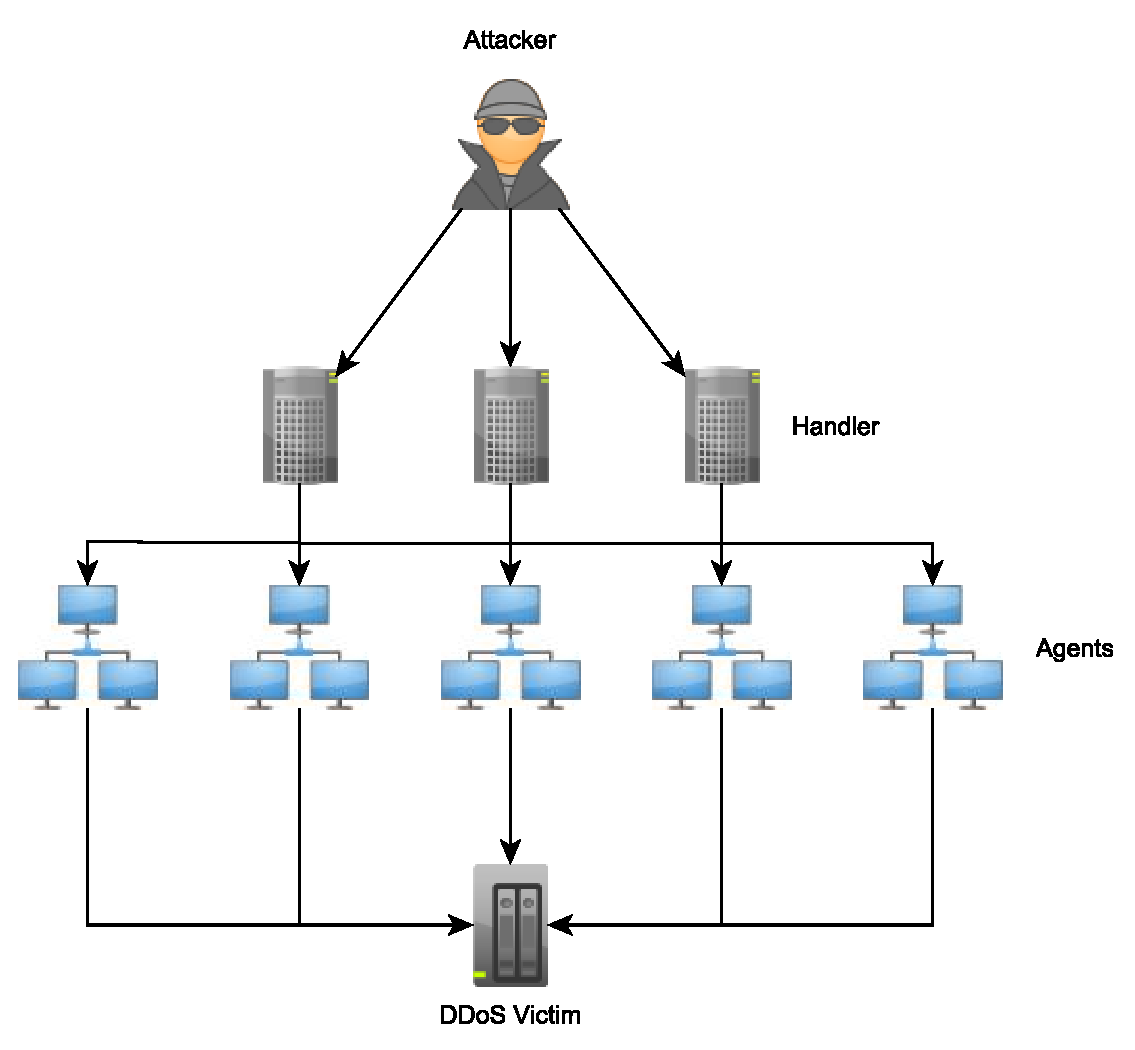
\includegraphics[width=\columnwidth]{section_2/Agent_Handler_Arch.eps}
    \caption{\gls{ddos} Agent-Handler Attack Model}
    \label{fig:Chap2_DDoS_Model}
\end{figure}

Specht  \textit{et al.}  \cite{specht2004distributed} created a \gls{dos} taxonomy to help classify various \gls{dos} attack
methods.  The taxonomy is depicted in Fig.~\ref{fig:Chap2_DDoS_Tax}.
According to Specht  \textit{et al.}\cite{specht2004distributed}, there are two primary classes of \gls{ddos}, namely \textit{bandwidth depletion} and \textit{resource depletion}.

\begin{figure}[h]
    \centering
    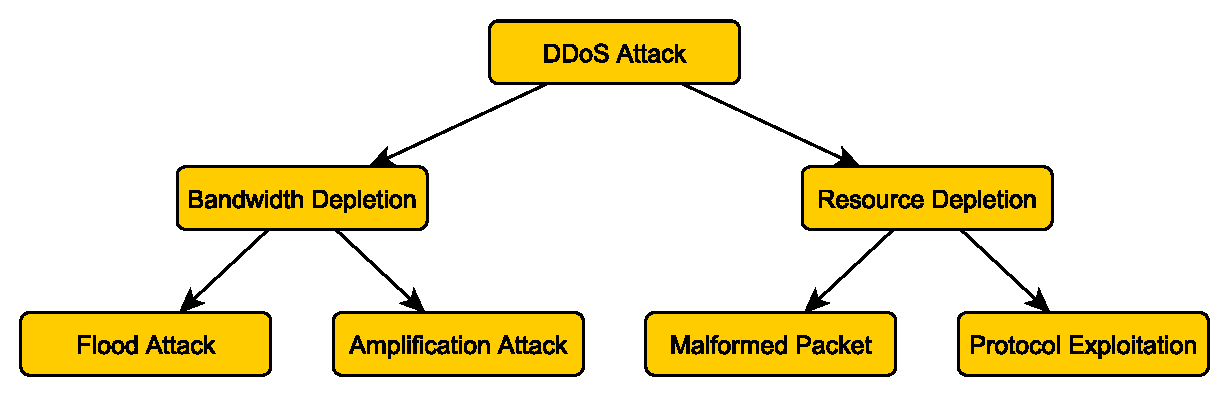
\includegraphics[width=\columnwidth]{section_2/DDoS_Taxonomy.eps}
    \caption{\gls{ddos} attack taxonomy  \cite{specht2004distributed}}
    \label{fig:Chap2_DDoS_Tax}
\end{figure}

Bandwidth depletion aims to deplete the network related resources of the victim. These attacks tend to generate large volumes of network traffic to deplete the bandwidth allocated to the victim's system. Resource depletion attacks aim to deplete the victim server's available resources rather than bandwidth.

Traditional amplification attacks leverage broadcast IP addresses to generate sufficient traffic to saturate the victim's bandwidth. The Smurf attack is an example of an amplification attack. The Smurf works by spoofing the IP address of the intended victim and then sending a ICMP\_ECHO\_REQUEST packet to a broadcast IP. The broadcast IP will broadcast the message to all the nodes within it's subnet, causing and amplification attack. The responses generated by the nodes, saturate the bandwidth of the victim server  \cite{kumar2007smurf}. According to Martin \textit{et al.}\cite{martin2002router} routers (as of 1999) no longer forward packets directed at their broadcast addresses. This means that most modern networks should be immune to Smurf attacks.

A \gls{drdos} attack is a modern variant of amplification attacks which uses vulnerable protocols or methods within protocols to generate large volumes of response traffic from legitimate service providers. This type of attack spoofs the IP address of the intended victim and performs a service request to the service provider using the spoofed IP address of the intended victim. The attack is known as a reflective attack because the response is ``reflected'' back to the victim IP address.  The \gls{udp} transportation layer protocol is often used to perform \gls{drdos} attacks due to lack of verification handshake in the \gls{udp} protocol  \cite{USCert2018}. By spoofing the IP address of the intended victim, neither the victim nor the service provider knows the true IP address of the attacker  \cite{USCert2018}.

An example of a \gls{drdos} attack is \gls{ntp} amplification. \gls{ntp} is an Internet protocol which is used to synchronise various web servers  \cite{RFC5905}.  The \gls{ntp} protocol has a method called $mon\_getlist$. By calling this method using the \gls{ntp} protocol, the service provider will respond with a list of \gls{ntp} response messages. The network traffic generated to make the $mon\_getlist$ request is significantly lower than the network traffic generated as a response \cite{czyz2014taming}. This is known as the amplification factor. Table~\ref{tab:2Amplify} provides the amplification factor for various protocols \cite{USCert2018}.

\begin{table}[h]
\centering
\caption{Amplification factor of various \gls{drdos} attacks \cite{USCert2018}}
\label{tab:2Amplify}
\begin{tabular}{| l | c | l | c |}
\hline
\textbf{Protocol}                                              & \textbf{\begin{tabular}[c]{@{}l@{}}Amplifica- \\ tion Factor\end{tabular}} & \textbf{Protocol}                                                & \textbf{\begin{tabular}[c]{@{}l@{}}Amplifica- \\ tion Factor\end{tabular}} \\ \hline
DNS                                                            & 28-54                                                                 & NTP                                                              & 556.9                                                                    \\ \hline
SNMPv2                                                         & 6.3                                                                      & NetBIOS                                                          & 3.8                                                                      \\ \hline
SSDP                                                           & 30.8                                                                     & CharGen                                                          & 358.8                                                                    \\ \hline
QOTD                                                           & 140.3                                                                    & Bit Torrent                                                      &                 3.8                                                         \\ \hline
\begin{tabular}[c]{@{}l@{}}Multicast DNS\\ (mDNS)\end{tabular} & 2-10                                                                  & \begin{tabular}[c]{@{}l@{}}Quake Network\\ Protocol\end{tabular} & 63.9                                                                     \\ \hline
Steam Protocol                                                 & 5.5                                                                      & Kad                                                              & 16.3                                                                     \\ \hline
RIPv1                                                          & 131.24                                                                   & \begin{tabular}[c]{@{}l@{}}Portmap\\ (RPCbind)\end{tabular}      & 7-28                                                                  \\ \hline
LDAP                                                           & 46-55                                                                 & CLDAP                                                            & 56-70                                                                 \\ \hline
TFTP                                                           & 60                                                                       & Memcached                                                         & \begin{tabular}[c]{@{}l@{}}10 000-\\ 51 000\end{tabular}               \\ \hline
\end{tabular}
\end{table}

At the time of writing this paper, the Memcached protocol produces the largest amplification factor of all known vulnerable protocols, see Table~\ref{tab:2Amplify} for full list of known vulnerable protocols and their corresponding amplification factors. According to the US \gls{cert}  \cite{USCert2018}, Memcached  has an amplification factor of 10 000 to 51 000, this means that for every byte of data sent by the attacker, the Memcached service responds with between 10 to 51 kilobytes of data. A high amplification factor greatly reduces the number of bots required by the attacker to launch a successful \gls{ddos} attack. 

Memcached is a network service which allows network
applications to cache database query results on networked
host, similar to how a computer's cache memory stores data in a temporary cache
 \cite{fitzpatrick2004distributed}. Memcached operates on \gls{udp} port 11211. The Memcached service allows distributed clusters of computers to store frequently requested database query results on the Memcached server rather than requiring additional database look-ups to retrieve the data. Depending on the Memcached server setup large volumes of data can be stored in the Memcached cache. It is best practise to not allow Memcached servers to be accessable from outside an organisation's firewall as the Memcached service may expose sensitive data over the network  \cite{ranabahu2009best}. Unfortunately due to misconfiguration or neglect of best practises some Memcached services are exposed to the Internet.  

During a \gls{drdos} attack, the attacker spoofs the IP address of the intended victim. Using the spoofed address, the attacker, requests that a large portion (if not all) of the data stored within the Memcached cache be returned as a result to the spoofed IP address. This results in the victim machine receiving a large volume of unsolicited network traffic.  If the attacker performs enough requests on behalf of the victim, the victims network resources will become depleted and prevent the victim from delivering services to legitimate network users. 

In the next Section, the data collection environment used to detect and mitigate the Memcached attack will be discussed.



 
\section{Data collection and analysis environment overview}
\label{sec3}

The \gls{sanren} was conceptualised in 2003 and implemented by the Meraka Institute of the \gls{csir} under contract to the \gls{dst} from 2008 onwards  \cite{draai2015implementing}. 


The \gls{sanren} network has approximately one million users spread across 151 sites throughout South Africa. The \gls{sanren} has a national backbone capacity of 10 Gbps. Typical client hand off is 1 Gbps though some main campuses connect at 10 Gbps. The average bandwidth per site is 2.82 Gbps. Fig.~\ref{fig:SANREN_net} depicts the high-level network architecture of the \gls{sanren} network  \cite{draai2015implementing}. The \gls{sanren} network has two main connection points to the international Internet infrastructure, namely SEACOM and \gls{wacs} \cite{draai2015implementing}.

\begin{figure}[h]
    \centering
    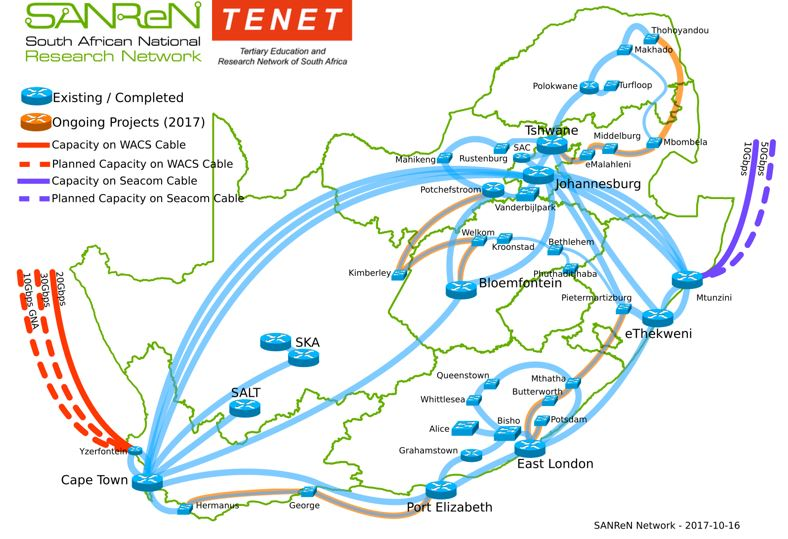
\includegraphics[width=\columnwidth]{section_3/SANREN_Net.JPG}
    \caption{\gls{sanren} network layout \cite{draai2015implementing}}
    \label{fig:SANREN_net}
\end{figure}

The size and scope of the \gls{sanren} infrastructure makes detecting and responding to network attacks challenging. Various sensors have been deployed on the \gls{sanren} to assist with detecting malicious activity.


These sensors include:
\begin{itemize}
    \item Network honeypots -- A honeypot is a closely monitored network decoy   \cite{mokube2007honeypots}. A honeypot can be a virtualised or physical replica of a networked service or infrastructure component. The goal of a honeypot is to act as a distraction for an attacker. A honeypot usually possesses several logging and measurement capabilities to capture the activities performed by the attacker on the decoy  \cite{spitzner2003honeypots2}.
    \item Network telescopes -- A network telescope is an unallocated IP address space which has some form of packet capture mechanism attached to it. Since the IP address space is unallocated, any packet which is routed to the address space is either a broadcast package, misconfigured host, network probe/scans, or potentially a malicious software seeking to spread across the network  \cite{irwin2012network}.
    \item Network flow collectors -- A network flow collector collects the bi-directional meta data of a network connection stream \cite{Graham2017Primer}.
\end{itemize}
For this paper only the network flow collection data is used for analysis due to privacy concerns and data availability. 


The \gls{sanren} \gls{csirt} uses NetFlow v9 (RFC 7011 \cite{RFC7011}) sensors to collect network flow data for traffic analysis and anomaly detection. NetFlow is a data model originally proposed by Cisco in 1996, to capture network flow information  \cite{Graham2017Primer}.  Network flow data is a representative model of the network traffic being transferred over the network. At the bare minimum a flow can be captured as a 6-tuple of information elements: source IP address, destination IP address, source port, destination port, protocol used and time-stamp  \cite{dietz2013passive}. NetFlow v9 does provide the option to add additional data element templates to the data model but for this analysis these additional templates are not required.

The main benefits of using  network flows as a means to detect cyber
incidences over traditional packet capture techniques is the speed at which network flow traffic can be captured. NetFlow is a high speed flow export protocol and thus presents less of a bottle neck for network data collection than traditional packet capture technologies  \cite{hofstede2014flow}.

Another benefit of flow-based data capture over packet capture techniques is the reduced privacy concerns. NetFlow only collects meta data related to the network traffic flow, it does not collect the data packet content \cite{hofstede2014flow}. 

A side effect of only capturing flow meta data is that packet payloads and specific packet signatures can not be detected using NetFlow. Based on the taxonomy of \gls{dos} attacks, presented by Specht \textit{et al.} \cite{specht2004distributed}, network flow analysis is best suited for detecting Bandwidth depletion attacks rather than Resource depletion attacks. Resource depletion attacks tends to exploit weakness with network protocols or inject malicious packet payloads into the network  \cite{specht2004distributed}.

The \gls{sanren} \gls{csirt} collects network flow data from various network exchange points throughout South Africa. The two primary network flow collection points are located at the \gls{wacs} and SEACOM connection points to the SANReN network. The routers at these collection points export all network flow data originating from or destined to the international IP address space, to a centralised NetFlow Collector. On average each of these collection nodes collects 20 Gigabytes of NetFlow data per day. Once the Netflow data has been exported. The flow data is analysed by the \gls{sanren} \gls{csirt} NetFlow Analyser system. If the analysis system detects any abnormal traffic an alert is generated and the \gls{sanren} \gls{csirt} is tasked to investigate the anomaly.

In Section~\ref{sec4} the data collected from these network flow collectors is used to detect the Memcached attack.


\section{Analysis of Memcached attack phases}
\label{sec4}

Due to the size and scope of the \gls{sanren} network, the \gls{sanren} \gls{csirt} is notified of multiple attacks on a regular basis. This attack analysis will focus specifically on the Memcached attack and how the attack was  observed and mitigated within the \gls{sanren} environment.



\textit{Figure~\ref{fig:time_line}} depicts the time-line of the Memcached attack. On 22 February 2018, the US-\gls{cert} sent out an alert sating that the Memcached protocol is vulnerable to \gls{drdos} attacks   \cite{USCert2018}. According to \cite{Akamai2018Memcached}, the attack reached its peek on 28 February 2018. According to \cite{DDoSMon}, a \gls{ddos} monitoring company, the Memcached attacks started drastically decreasing in size from 6 March 2018.

\begin{figure}[h]
    \centering
    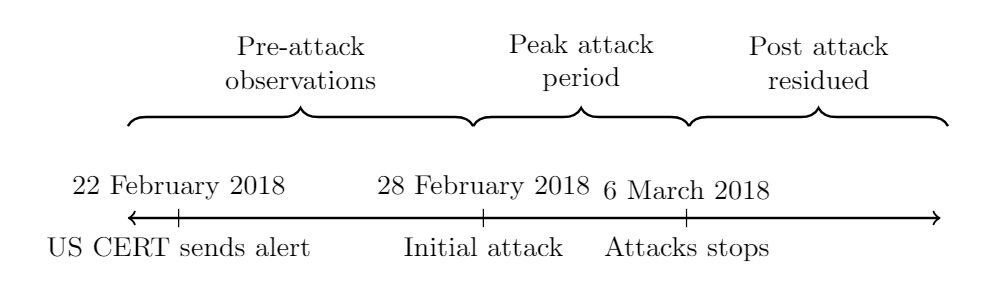
\includegraphics[width=\columnwidth]{section_4/memcached_phases.JPG}
    \caption{Memcached attack time-line}
    \label{fig:time_line}
\end{figure}

In the remainder of this sub-section the various phases of the attack will be analysed using the network flow data obtained from the \gls{sanren} NetFlow collector.

\subsection{Pre-attack observations}
\label{sub-pre-attack}

Once the security alert was posted by the US-\gls{cert}, the \gls{sanren} \gls{csirt} modified the network flow analysis system to notify the CSIRT if any anomalies are detected on port 11 211, the default Memcached service port. The CSIRT also identified all active Memcached servers on the \gls{sanren} network using the NetFlow data set. Prior to the initial attack only four Memcached servers were detected.



Prior to the Memcached attack disclosure, the \gls{sanren} network observed approximately 2.8 Megabytes of data, resulting from 917 flows per day\footnote{Average data rate observed for period 1 January 2018 -- 10 February 2018}. In \textit{Figures~\ref{fig:pre_graph_bytes}--~\ref{fig:pre_graph_bpf}}, three graphs are presented representing the Memcached traffic observed prior to the primary attack date. The first graph depicts the traffic in bytes observed during this period, the second graph plots the number of flows observed and the third graph plots the \gls{bpf} for the period.

\begin{figure}
    \centering
    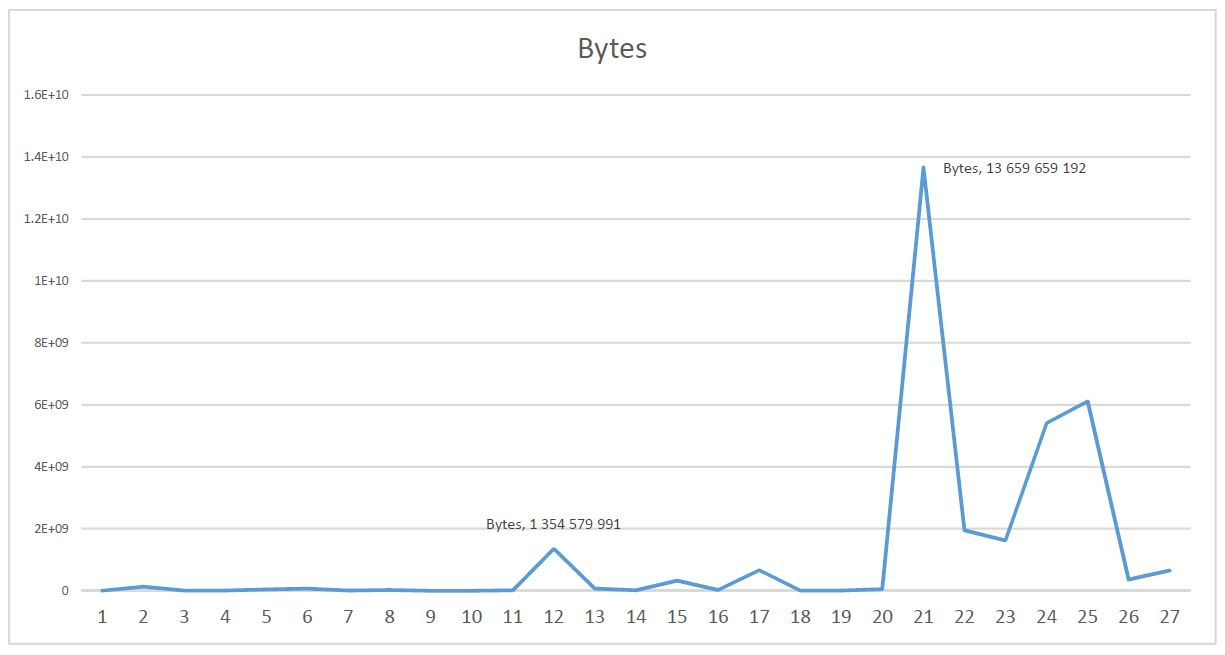
\includegraphics[width=\columnwidth]{section_4/memcached_pre-attack_bytes.JPG}
    \caption{Pre-attack Memcached protocol activity bytes observed}
    \label{fig:pre_graph_bytes}
\end{figure}

\begin{figure}
    \centering
    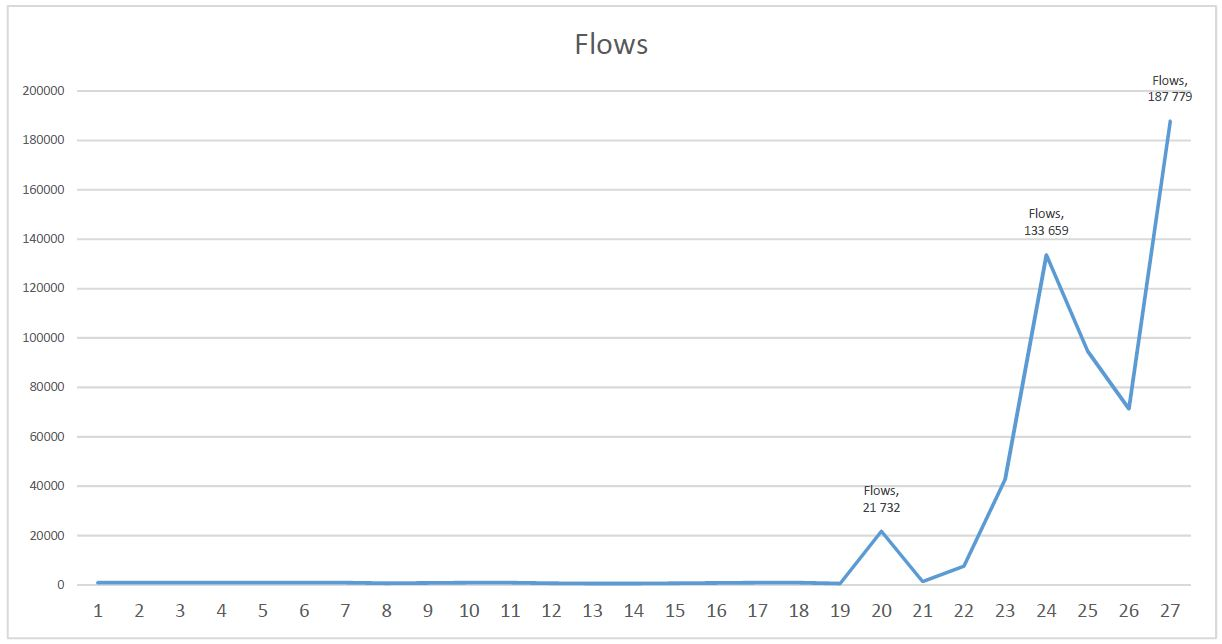
\includegraphics[width=\columnwidth]{section_4/memcached_pre-attack_flows.JPG}
    \caption{Pre-attack Memcached protocol activity flows observed }
    \label{fig:pre_graph_flows}
\end{figure}

\begin{figure}
    \centering
    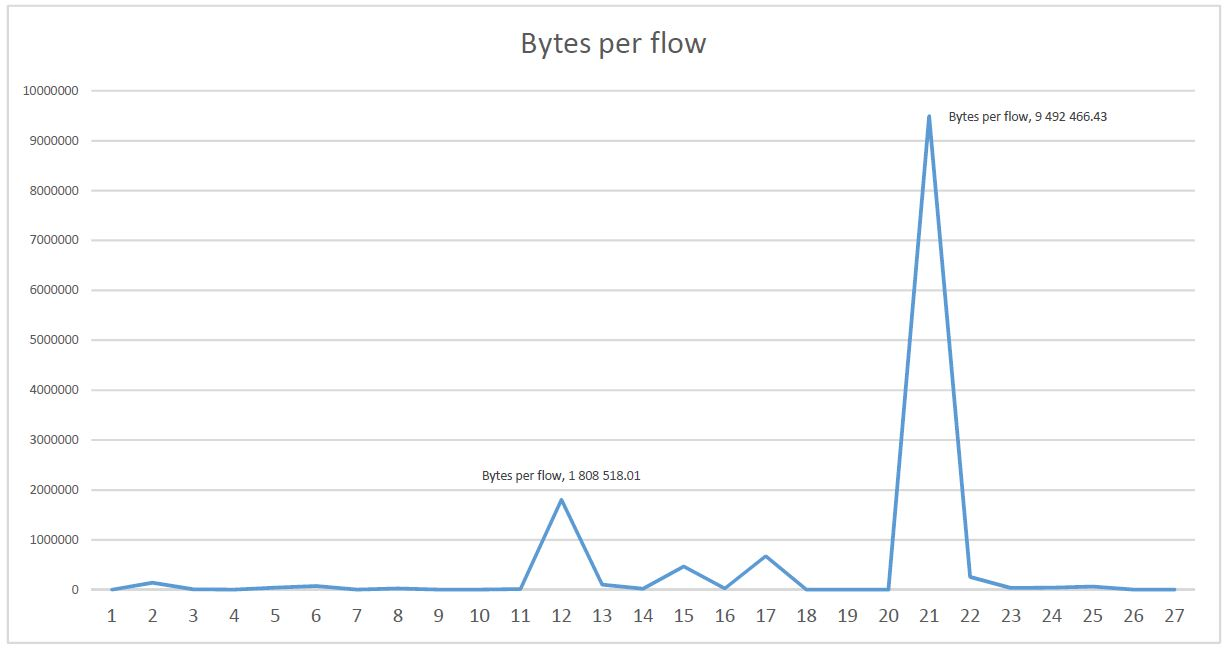
\includegraphics[width=\columnwidth]{section_4/memcached_pre-attack_bpf.JPG}
    \caption{Pre-attack Memcached protocol activity bytes per flow observed }
    \label{fig:pre_graph_bpf}
\end{figure}
In the first graph, \textit{Figure~\ref{fig:pre_graph_bytes}}, a large spike in network traffic is observed (13 Gigabyte in one day) on 21 February 2018, the day before the US-\gls{cert} sent out the advisory. A smaller increase in bandwidth usage can also be observed on 12 February 2018 (1.3 Gigabyte of data). 



In the second graph, \textit{Figure~\ref{fig:pre_graph_flows}}, it is shown that the number of flows associated with the Memcached service greatly increased since 23 February. Despite the increase in the number of flows, the data usage did not increase at a similar rate, to that of the flow count. The number of flows per day increase by 20 000 \%, from an average of 939 to a maximum of 187 779. Unlike in graph one, the number of flows did not have a notable increase on 12 February. 



In the third graph, \textit{Figure~\ref{fig:pre_graph_bpf}}, there is a noticeable increase in \gls{bpf} observed on 21 February 2018. A sudden increase in \gls{bpf} is an indicator for amplification. The \gls{bpf} graph indicates that amplification traffic was observed before the US-\gls{cert} sent out the alert. On average the Memcached service produced a 30 Kilobyte response per flow, prior to the vulnerability disclosure. On 21 February, 9.5 Megabyte of data was generated per flow.  

Based on the NetFlow sensor analysis the majority of the flows observed between 23 February 2018 and 27 February 2018, were as a result of port scans and service discovery scans. These flows represent 93.7 \% of all flows observed in this period. The observed service discovery flows exhibit the following properties:
\begin{itemize}
    \item Destination port 11 211 (Memcached),
    \item \gls{udp} protocol,
    \item Memcached request flow, payload size  \textless 49 bytes.
    \item Memcached response flow, payload size  \textless 107 bytes.
    \item Source IP distribution:   185.176.192.244 (40.6\%),  185.94.111.1 (21.5\%),\newline  185.194.112.10 (16.5\%) and other (21.4\%)\footnote{Due to IP spoofing, the source IP detected by the network flow sensor may be inaccurate \cite{senie1998network}.}.
\end{itemize}

\subsection{Peak attack period}
\label{sub-during-attack}

According to \cite{Akamai2018Memcached}, the primary Memcached attack period was between 28 February 2018 and 6 March 2018. During the peak traffic period, five Memcached servers were observed.

According to \cite{Shodan}, a search engine for vulnerable Internet-connected devices, there were 87 811 Internet facing Memcached servers worldwide on 28 March 2018. Of all the servers observed, only 212 of these servers were located within South Africa and only 4 were hosted by \gls{sanren}.


At 8 AM SAST, 1 March 2018, the \gls{sanren} \gls{csirt} were notified of the sudden increase in Memcached activity and by 9H30 AM SAST, 1 March 2018, the four servers which were observed during the pre-attack phase were patched. Memcached request messages were still received by the servers, but no Memcached responses were issued to servers outside the local network IP address ranges. On 2 March 2018 a fifth Memcached server became active on the \gls{sanren} network. Due to the servers limited bandwidth it produced significantly less traffic than the initial four servers.  

\textit{Table~\ref{tab:memcached_sum}} summarises the average data flow activity observed by the \gls{sanren} network flow collector for this period. The server IP addresses and host names have been anonymised to protect the \gls{sanren} users.

% \begin{figure}
%     \centering
%     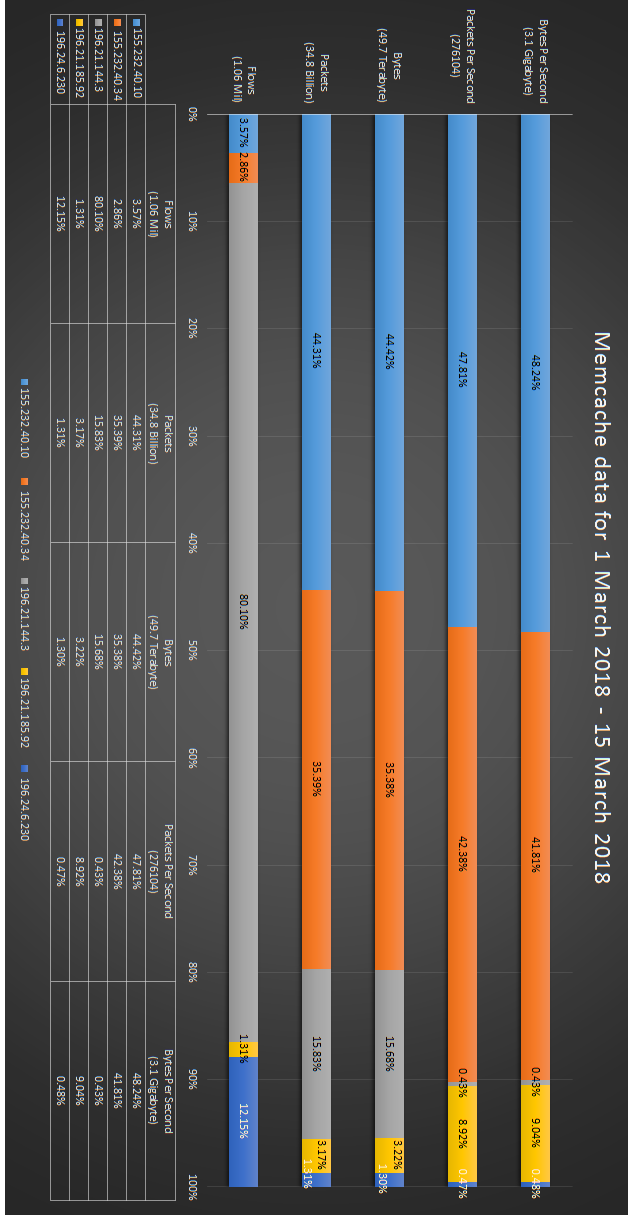
\includegraphics[width=\columnwidth]{section_4/Memcached_march_2018.png}
%     \caption{Memcached data for March 2018}
%     \label{fig:4memcached}
% \end{figure}


\begin{table}[h]
\caption{Summary of \gls{ddos} activity observed during peak attack period}
\label{tab:memcached_sum}
\begin{tabular}{l|r|r|r|r|r|}
\cline{2-6}
                              & \multicolumn{1}{l|}{Flows} & \multicolumn{1}{l|}{Packets} & \multicolumn{1}{l|}{Bytes} & \multicolumn{1}{l|}{\begin{tabular}[c]{@{}l@{}}Packets \\ /second\end{tabular}} & \multicolumn{1}{l|}{\begin{tabular}[c]{@{}l@{}}Bytes \\ /second\end{tabular}} \\ \hline
\multicolumn{1}{|l|}{Server 1} & $38 076$                   & $1.54e+10$                   & $2.12e+13$                 & $132 005$                                                                       & $1.5e+9$                                                                      \\ \hline
\multicolumn{1}{|l|}{Server 2} & $30 470$                   & $1.23e+10$                   & $1.76e+13$                 & $117 001$                                                                       & $1.3e+9$                                                                      \\ \hline
\multicolumn{1}{|l|}{Server 3} & $853 755$                  & $5.5e+9$                     & $7.8e+12$                  & $1 177$                                                                         & $1.33e+7$                                                                     \\ \hline
\multicolumn{1}{|l|}{Server 4} & $13 970$                   & $1.1e+9$                     & $1.6e+12$                  & $24 616$                                                                        & $2.81e+8$                                                                    \\ \hline
\multicolumn{1}{|l|}{Server 5} & $129 528$                  & $4.55e+8$                    & $1.6e+12$                  & $1 305$                                                                         & $1.49e+7$                                                                     \\ \hline
\multicolumn{1}{|l|}{Total}    & $1.06e+6$                  & $3.48e+10$                   & $4.97e+13$                 & 276 104                                                                         & $3.1e+9$                                                                      \\ \hline
\end{tabular}
\end{table}

% \begin{table*}[]
% \caption{Summary of \gls{ddos} activity observed during peak attack period}
% \label{tab:memcached_sum}
% \begin{tabular}{l|r|r|r|r|r|}
% \cline{2-6}
%                               & \multicolumn{1}{l|}{Flows} & \multicolumn{1}{l|}{Packets} & \multicolumn{1}{l|}{Bytes} & \multicolumn{1}{l|}{\begin{tabular}[c]{@{}l@{}}Packets \\ /second\end{tabular}} & \multicolumn{1}{l|}{\begin{tabular}[c]{@{}l@{}}Bytes \\ /second\end{tabular}} \\ \hline
% \multicolumn{1}{|l|}{Server 1} & \num{38 076}                   & \num{1.54e+10}                   & \num{2.12e+13}                 & \num{132 005}                                                                       & \num{1.5e+9}                                                                      \\ \hline
% \multicolumn{1}{|l|}{Server 2} & \num{30 470}                   & \num{1.23e+10}                   & \num{1.76e+13}                 & \num{117 001}                                                                       & \num{1.3e+9}                                                                      \\ \hline
% \multicolumn{1}{|l|}{Server 3} & \num{853 755}                  & \num{5.5e+9}                     & \num{7.8e+12}                  & \num{1 177}                                                                         & \num{1.33e+7}                                                                     \\ \hline
% \multicolumn{1}{|l|}{Server 4} & \num{13 970}                   & \num{1.1e+9}                     & \num{1.6e+12}                  & \num{24 616}                                                                        & \num{2.81e+8}                                                                    \\ \hline
% \multicolumn{1}{|l|}{Server 5} & \num{129 528}                  & \num{4.55e+8}                    & \num{1.6e+12}                  & \num{1 305}                                                                         & \num{1.49e+7}                                                                     \\ \hline
% \multicolumn{1}{|l|}{Total}    & \num{1.06e+6}                  & \num{3.48e+10}                   & \num{4.97e+13}                 & \num{276 104}                                                                         & \num{3.1e+9}                                                                      \\ \hline
% \end{tabular}
% \end{table*}





Over the 6 day period 49.7 Terabytes of data was generated by the Memcached servers of which 48.6 Terabytes were transmitted between 10 PM SAST, 28 February 2018 and 10 AM SAST, 1 March 2018. At its peek, Server 1 and Server 2 each produced 10.9 Gigabytes of traffic per second. The Memcached attack completely saturated the bandwidth allocated to Server 1 and Server 2. Server 1 and Server 2 only contributed to 6.43\% of the data flows observed during this period, but they contributed to 79.8\% of the traffic generated. On average, each flow generated by Server 1 and Server 2 produced 46.8 Megabytes of traffic. This is a significant increase from the 30 Kilobyte responses observed during the pre-attack observations. The average amplification factor observed by these servers were 1:49500.

Server 3 only had a one Megabyte connection with a four Megabyte Memcached cache. Due to Server 3's limited resources it produced significantly less response traffic than Server 1 and Server 2 despite receiving 80.1\% of the observed Memcached request flows. Server 4 had a 24 Megabyte bandwidth with a 64 Kilobyte Memcached cache. Though Server 4 had more bandwidth capacity than Server 3, it produced far less traffic than $Server 3$ due to the small cache size. The amplification factor of Server 4 was also the lowest of all observed servers due to the reduced cache size, only 1:1600. 

The \gls{sanren} \gls{csirt} applied software patches to Server 1 to 4 on 1 March 2018 at 10 AM SAST. Since the patches were applied, the servers still receive periodic service discovery probes and Memcached requests but they no longer respond to unverified requests.

Server 5's Memcached service only became active on 2 March 2018. Server 5 only had a one Megabyte international connection and a 128 Kilobyte Memcached cache. The server operator was not aware of the Memcached service being enabled on their server. The server only generated traffic directed at seven target IP addresses. According to the network flow data, Server 5 was also the victim of a brute force \gls{ssh} attack prior to the Memcached service starting up. Server 5 was not managed by the \gls{sanren} network operators, but by a private University systems administrator. Given the suspicious behaviour observed on Server 5, the \gls{sanren} \gls{csirt} notified the system administrator of the server and provided them with an analysis of the server's behaviour. 


An increase in the number of Memcached severs also increased world wide after the peek periods of attack. On 28 February, there were 214 South African and 87 811 international servers vulnerable to Memcached amplification, according to \cite{Shodan}. On 4 March 2018, the number of vulnerable servers in South Africa reached its peek, 236. At least 8 of the newly discovered South African servers were confirmed to be Honey Pots. The international vulnerable server count reached its peek on 7 March 2018, with 107 431 according to SHODAN's reporting tools  \citep{Shodan}. The international server count increased by 22.3\% during the attack period, thus far no information has been released as to how many of these server are Honey Pots.    

\cite{CyberReason},  discovered that attackers were embedding ransomware notes into the Memcached payloads. Figure.~\ref{fig:ransom} illustrates a sample payload. In the payload message the attacker requests the victim to pay 50 Monero, a crypto currency, into a crypto wallet account. According to Kerb \cite{kerbs2018Powerful} it is not clear if any victim's paid the ransom amount. The US-CERT and Cyber Reason warned victims not to pay the ransom since there was no guarantee that attacks would stop after the payment was made \citep{kerbs2018Powerful,CyberReason}.

\begin{figure}[H]
    \centering
    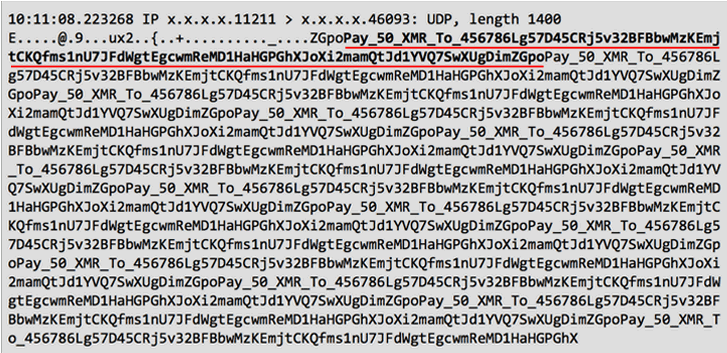
\includegraphics[width=\columnwidth]{section_4/ransom_memcached.PNG}
    \caption{Sample ransomware message in Memcached payload}
    \label{fig:ransom}
\end{figure}


\subsection{Post attack residue}
\label{sub-post-attack}


During the attack period 12 139 unique IP addresses were observed to be communicating over port 11 211 using the Memcached protocol on the \gls{sanren} network. As part of the post attack analysis, the network flow data was used to filter potential attack IP addresses from the victim IP addresses\footnote{It should be noted that,  IP addresses can be spoofed when using \gls{udp} traffic \cite{senie1998network}.}.  As part of our classification several metrics were defined to either include or exclude a candidate IP address as an attacker or victim. These criteria are as follows:
\begin{itemize}
    \item If the IP address belongs to a known legitimate user of Memcached service, label the IP as $benign$. 
    \item If the number of Memcached requests issued per day increased by more than 50\% after 21 February, the IP was labelled as $suspicious$.
    \item If the ratio of request traffic to response traffic generated by the IP was greater than 1:100, the IP was labelled as a $victim$.
    \item If any of the other network flow sensors\footnote{The sensor to detect port scanning activity is based on the \gls{taps} algorithm, proposed by \cite{sridharan2006connectionless}. \gls{taps} port scan detection technique will be discussed in greater detail in sub-section \ref{sec4_port_scan}.}, deployed by the \gls{sanren} \gls{csirt}, detected the IP as a port scanner, the IP was labelled as a $port\_scanner$. 
    \item If any of the the $port\_scanner$ IP addresses were found to only be scanning for port 11 211 and using the Memcached protocol, it was assigned an additional label, $memcached\_scanner$. 
\end{itemize}
\textit{Table~\ref{tab:IP_sum}} summarises labels assigned to IP addresses during each phase.

\begin{table}[h]
\caption{Summary of IP addresses observed during Memcached attack}
\label{tab:IP_sum}
\begin{tabular}{l|r|r|r|r|r|}
\cline{2-6}
                                                                             & \multicolumn{1}{l|}{Observed} & \multicolumn{1}{l|}{Benign} & \multicolumn{1}{l|}{\begin{tabular}[c]{@{}l@{}}Port\\ Scanner\end{tabular}} & \multicolumn{1}{l|}{\begin{tabular}[c]{@{}l@{}}Memcached\\ Scanner\end{tabular}} & \multicolumn{1}{l|}{Victim} \\ \hline
\multicolumn{1}{|l|}{\begin{tabular}[c]{@{}l@{}}Pre-\\ attack\end{tabular}}  & 116                           & 17                          & 88                                                                          & 31                                                                               & 39                          \\ \hline
\multicolumn{1}{|l|}{\begin{tabular}[c]{@{}l@{}}Peak-\\ attack\end{tabular}} & 12 116                        & 17                          & 4 116                                                                       & 1 012                                                                            & 738                         \\ \hline
\multicolumn{1}{|l|}{\begin{tabular}[c]{@{}l@{}}Post-\\ attack\end{tabular}} & 378                           & 16                          & 279                                                                         & 201                                                                              & 0                           \\ \hline
\end{tabular}
\end{table}


During the pre-attack phase only 116 unique IP addresses were observed. Of the 116, only 17 were labelled $benign$ since they belong to verified users which use the Memcached service on a regular basis. 39 IP addresses were labelled as $victims$. 88 IP addresses were labelled as $port\_scanners$ and 31 of the $port\_scanners$ IP addresses were labelled as $memcached\_scanners$. 3 of the IP addresses labelled as $victim$ also had the label $memcached\_scanner$ associated with it. This may indicate that the attackers were testing the exploit against their own systems prior to launching the main attack. 12 IP addresses had 5 or less network flows associated with the IP and could not be classified using any of the labels defined.


\begin{figure}[]h]
    \centering
    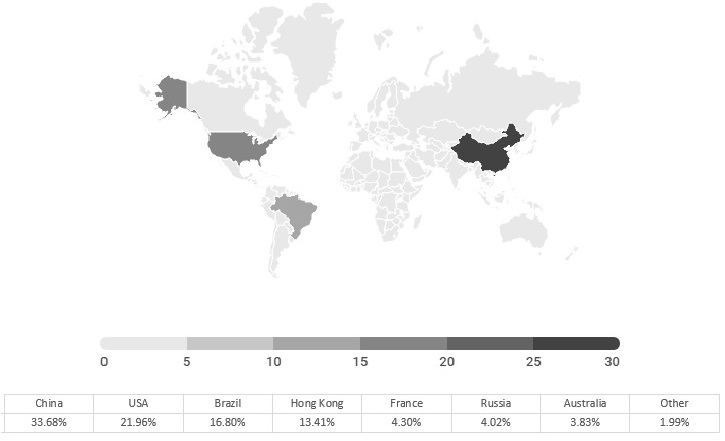
\includegraphics[width=\columnwidth]{section_4/map_countries_memcahced.jpg}
    \caption{Distribution of Memcached \gls{drdos} victims}
    \label{fig:map}
\end{figure}

During the peek period of attack 12 116 unique IP addresses were observed. 8 738 IP addresses received amplified Memcached traffic and were labelled $victim$ as a result. Only 371 of the victim IP addresses received over one Gigabyte per second traffic flows. \textit{Figure~\ref{fig:map}} depicts the global distribution of Memcached \gls{drdos} victims. 4 116 IP addresses were labelled as $port\_scanners$, 881 of which were $memcached\_scanners$. 1 012 IP address had less than 5 flows associated with the Memcached service and were not classified by the network flow sensors.

During the post attack phase only 378 unique IP Addresses were detected by the network flow sensor. Due to the \gls{sanren} servers being patched, no IP addresses were labelled as $victims$ during the post attack phase. This confirms that the software patch did prevent any further \gls{drdos} attacks. 279 IP addresses were found to be performing port scans and 201 were found to be scanning port 11 211 specifically. 191 of the IP addresses labelled as $memcached\_scanners$ did not appear in the list of $memcached\_scanners$ obtained in the pre-attack phase. 29 IP addresses did not produce enough network flow data for classification.

From the post analysis it is clear that the majority of Memcached attack activity has subsided. The analysis also confirmed that the software patches prevented further amplification attacks.



\section{Conclusion and recommendations}
\label{sec5}

In this paper NetFlow logs were used to analyse the effect of the Memcached \gls{drdos} attack on the \gls{sanren} infrastructure. Metrics from each phase of the attack was used to show the progression of the attack traffic over time, as well as the effect of applying software patches to the vulnerable systems. Sensors and classifiers developed during this research have been added to the \gls{sanren} \gls{csirt} tool-set for future attack analysis. 

This paper showed how network flow analysis could be used to perform a post attack investigation and identify potential victims and aggressors. Network flow analysis identified key indicators for amplification attacks by providing the researchers a mechanism to compare data amplification ratios and provide alerts for possible amplification attacks. It is recommended that \gls{udp} traffic should be monitored for possible amplification attacks in future. All \gls{drdos} attacks listed by the US-\gls{cert}  \cite{USCert2018} utilise \gls{udp} traffic amplification. Due to \gls{udp}'s lack of source IP address verification, attribution of aggressors is speculative.


%
\section{Introduction}
\label{sec:intro}


The \gls{sanren} \gls{csirt} supports research and education institutions within South Africa by providing security awareness training, security alerts, incident handling and knowledge sharing opportunities to the \gls{sanren} community. The \gls{sanren} \gls{csirt} is tasked with detecting network attacks and anomalies on the \gls{sanren} network and providing constituents with advice and recommended response actions to mitigate malicious activity (which could lead to cyber security incidents).

On 28 February 2018 the world's larges \gls{ddos} attack was detected by Akamai, a \gls{ddos} mitigation firm \cite{kerbs2018Powerful}. According to Akamai the attack reached a peak of 1.3 \gls{tbps} against one of their clients\cite{Akamai2018Memcached}. The attackers used a reflective amplification attack, also known as a \gls{drdos}, to attack their targets. A \gls{drdos} attack uses weaknesses within various Internet protocols to generate large volumes of network traffic from trusted service providers \cite{gibson2002distributed}.  During the attack, the attackers used services exposed via the \gls{sanren} network to amplify their network traffic, causing a \gls{ddos} attack against their intended targets. A detailed description of the \gls{drdos} attack methodology and its impact will be presented in Section \ref{sec2}.

Mitigation and detection techniques can be developed by analysing the behavioural pattern of these attacks. In this paper a postmortem analysis of the Memcached \gls{drdos} attack will be provided. The analysis will focus on the various phases of the attack and the steps taken by the \gls{sanren} \gls{csirt} to detect and mitigate the effect of the attack.

 This paper is structured as follows. In Section \ref{sec2} an overview of \gls{drdos} attacks will be provided. The basic attack structure and methodology will be covered. In Section \ref{sec3} our analysis environment and data capture methodology will be described. In Section \ref{sec4} the attack phases of the Memcached attack will be analysed. In Section \ref{sec5} the conclusion and recommendation for future attack detection will be presented.





\section{Introduction}

The \textit{proceedings} are the records of a conference.\footnote{This
  is a footnote}  ACM seeks
to give these conference by-products a uniform, high-quality
appearance.  To do this, ACM has some rigid requirements for the
format of the proceedings documents: there is a specified format
(balanced double columns), a specified set of fonts (Arial or
Helvetica and Times Roman) in certain specified sizes, a specified
live area, centered on the page, specified size of margins, specified
column width and gutter size.

\section{The Body of The Paper}
Typically, the body of a paper is organized into a hierarchical
structure, with numbered or unnumbered headings for sections,
subsections, sub-subsections, and even smaller sections.  The command
\texttt{{\char'134}section} that precedes this paragraph is part of
such a hierarchy.\footnote{This is a footnote.} \LaTeX\ handles the
numbering and placement of these headings for you, when you use the
appropriate heading commands around the titles of the headings.  If
you want a sub-subsection or smaller part to be unnumbered in your
output, simply append an asterisk to the command name.  Examples of
both numbered and unnumbered headings will appear throughout the
balance of this sample document.

Because the entire article is contained in the \textbf{document}
environment, you can indicate the start of a new paragraph with a
blank line in your input file; that is why this sentence forms a
separate paragraph.

\subsection{Type Changes and {\itshape Special} Characters}

We have already seen several typeface changes in this sample.  You can
indicate italicized words or phrases in your text with the command
\texttt{{\char'134}textit}; emboldening with the command
\texttt{{\char'134}textbf} and typewriter-style (for instance, for
computer code) with \texttt{{\char'134}texttt}.  But remember, you do
not have to indicate typestyle changes when such changes are part of
the \textit{structural} elements of your article; for instance, the
heading of this subsection will be in a sans serif\footnote{Another
  footnote here.  Let's make this a rather long one to see how it
  looks.} typeface, but that is handled by the document class file.
Take care with the use of\footnote{Another footnote.}  the
curly braces in typeface changes; they mark the beginning and end of
the text that is to be in the different typeface.

You can use whatever symbols, accented characters, or non-English
characters you need anywhere in your document; you can find a complete
list of what is available in the \textit{\LaTeX\ User's Guide}
\cite{Lamport:LaTeX}.

\subsection{Math Equations}
You may want to display math equations in three distinct styles:
inline, numbered or non-numbered display.  Each of
the three are discussed in the next sections.

\subsubsection{Inline (In-text) Equations}
A formula that appears in the running text is called an
inline or in-text formula.  It is produced by the
\textbf{math} environment, which can be
invoked with the usual \texttt{{\char'134}begin\,\ldots{\char'134}end}
construction or with the short form \texttt{\$\,\ldots\$}. You
can use any of the symbols and structures,
from $\alpha$ to $\omega$, available in
\LaTeX~\cite{Lamport:LaTeX}; this section will simply show a
few examples of in-text equations in context. Notice how
this equation:
\begin{math}
  \lim_{n\rightarrow \infty}x=0
\end{math},
set here in in-line math style, looks slightly different when
set in display style.  (See next section).

\subsubsection{Display Equations}
A numbered display equation---one set off by vertical space from the
text and centered horizontally---is produced by the \textbf{equation}
environment. An unnumbered display equation is produced by the
\textbf{displaymath} environment.

Again, in either environment, you can use any of the symbols
and structures available in \LaTeX\@; this section will just
give a couple of examples of display equations in context.
First, consider the equation, shown as an inline equation above:
\begin{equation}
  \lim_{n\rightarrow \infty}x=0
\end{equation}
Notice how it is formatted somewhat differently in
the \textbf{displaymath}
environment.  Now, we'll enter an unnumbered equation:
\begin{displaymath}
  \sum_{i=0}^{\infty} x + 1
\end{displaymath}
and follow it with another numbered equation:
\begin{equation}
  \sum_{i=0}^{\infty}x_i=\int_{0}^{\pi+2} f
\end{equation}
just to demonstrate \LaTeX's able handling of numbering.

\subsection{Citations}
Citations to articles~\cite{bowman:reasoning,
clark:pct, braams:babel, herlihy:methodology},
conference proceedings~\cite{clark:pct} or maybe
books \cite{Lamport:LaTeX, salas:calculus} listed
in the Bibliography section of your
article will occur throughout the text of your article.
You should use BibTeX to automatically produce this bibliography;
you simply need to insert one of several citation commands with
a key of the item cited in the proper location in
the \texttt{.tex} file~\cite{Lamport:LaTeX}.
The key is a short reference you invent to uniquely
identify each work; in this sample document, the key is
the first author's surname and a
word from the title.  This identifying key is included
with each item in the \texttt{.bib} file for your article.

The details of the construction of the \texttt{.bib} file
are beyond the scope of this sample document, but more
information can be found in the \textit{Author's Guide},
and exhaustive details in the \textit{\LaTeX\ User's
Guide} by Lamport~\shortcite{Lamport:LaTeX}.

This article shows only the plainest form
of the citation command, using \texttt{{\char'134}cite}.

Some examples.  A paginated journal article \cite{Abril07}, an enumerated
journal article \cite{Cohen07}, a reference to an entire issue \cite{JCohen96},
a monograph (whole book) \cite{Kosiur01}, a monograph/whole book in a series (see 2a in spec. document)
\cite{Harel79}, a divisible-book such as an anthology or compilation \cite{Editor00}
followed by the same example, however we only output the series if the volume number is given
\cite{Editor00a} (so Editor00a's series should NOT be present since it has no vol. no.),
a chapter in a divisible book \cite{Spector90}, a chapter in a divisible book
in a series \cite{Douglass98}, a multi-volume work as book \cite{Knuth97},
an article in a proceedings (of a conference, symposium, workshop for example)
(paginated proceedings article) \cite{Andler79}, a proceedings article
with all possible elements \cite{Smith10}, an example of an enumerated
proceedings article \cite{VanGundy07},
an informally published work \cite{Harel78}, a doctoral dissertation \cite{Clarkson85},
a master's thesis: \cite{anisi03}, an online document / world wide web
resource \cite{Thornburg01, Ablamowicz07, Poker06}, a video game (Case 1) \cite{Obama08} and (Case 2) \cite{Novak03}
and \cite{Lee05} and (Case 3) a patent \cite{JoeScientist001},
work accepted for publication \cite{rous08}, 'YYYYb'-test for prolific author
\cite{SaeediMEJ10} and \cite{SaeediJETC10}. Other cites might contain
'duplicate' DOI and URLs (some SIAM articles) \cite{Kirschmer:2010:AEI:1958016.1958018}.
Boris / Barbara Beeton: multi-volume works as books
\cite{MR781536} and \cite{MR781537}.

A couple of citations with DOIs: \cite{2004:ITE:1009386.1010128,
  Kirschmer:2010:AEI:1958016.1958018}.

Online citations: \cite{TUGInstmem, Thornburg01, CTANacmart}.


\subsection{Tables}
Because tables cannot be split across pages, the best
placement for them is typically the top of the page
nearest their initial cite.  To
ensure this proper ``floating'' placement of tables, use the
environment \textbf{table} to enclose the table's contents and
the table caption.  The contents of the table itself must go
in the \textbf{tabular} environment, to
be aligned properly in rows and columns, with the desired
horizontal and vertical rules.  Again, detailed instructions
on \textbf{tabular} material
are found in the \textit{\LaTeX\ User's Guide}.

Immediately following this sentence is the point at which
Table~\ref{tab:freq} is included in the input file; compare the
placement of the table here with the table in the printed
output of this document.

\begin{table}
  \caption{Frequency of Special Characters}
  \label{tab:freq}
  \begin{tabular}{ccl}
    \toprule
    Non-English or Math&Frequency&Comments\\
    \midrule
    \O & 1 in 1,000& For Swedish names\\
    $\pi$ & 1 in 5& Common in math\\
    \$ & 4 in 5 & Used in business\\
    $\Psi^2_1$ & 1 in 40,000& Unexplained usage\\
  \bottomrule
\end{tabular}
\end{table}

To set a wider table, which takes up the whole width of the page's
live area, use the environment \textbf{table*} to enclose the table's
contents and the table caption.  As with a single-column table, this
wide table will ``float'' to a location deemed more desirable.
Immediately following this sentence is the point at which
Table~\ref{tab:commands} is included in the input file; again, it is
instructive to compare the placement of the table here with the table
in the printed output of this document.


\begin{table*}
  \caption{Some Typical Commands}
  \label{tab:commands}
  \begin{tabular}{ccl}
    \toprule
    Command &A Number & Comments\\
    \midrule
    \texttt{{\char'134}author} & 100& Author \\
    \texttt{{\char'134}table}& 300 & For tables\\
    \texttt{{\char'134}table*}& 400& For wider tables\\
    \bottomrule
  \end{tabular}
\end{table*}
% end the environment with {table*}, NOTE not {table}!

It is strongly recommended to use the package booktabs~\cite{Fear05}
and follow its main principles of typography with respect to tables:
\begin{enumerate}
\item Never, ever use vertical rules.
\item Never use double rules.
\end{enumerate}
It is also a good idea not to overuse horizontal rules.


\subsection{Figures}

Like tables, figures cannot be split across pages; the best placement
for them is typically the top or the bottom of the page nearest their
initial cite.  To ensure this proper ``floating'' placement of
figures, use the environment \textbf{figure} to enclose the figure and
its caption.

This sample document contains examples of \texttt{.eps} files to be
displayable with \LaTeX.  If you work with pdf\LaTeX, use files in the
\texttt{.pdf} format.  Note that most modern \TeX\ systems will convert
\texttt{.eps} to \texttt{.pdf} for you on the fly.  More details on
each of these are found in the \textit{Author's Guide}.

\begin{figure}
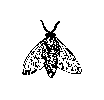
\includegraphics{fly}
\caption{A sample black and white graphic.}
\end{figure}

\begin{figure}
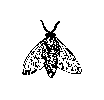
\includegraphics[height=1in, width=1in]{fly}
\caption{A sample black and white graphic
that has been resized with the \texttt{includegraphics} command.}
\end{figure}


As was the case with tables, you may want a figure that spans two
columns.  To do this, and still to ensure proper ``floating''
placement of tables, use the environment \textbf{figure*} to enclose
the figure and its caption.  And don't forget to end the environment
with \textbf{figure*}, not \textbf{figure}!

\begin{figure*}
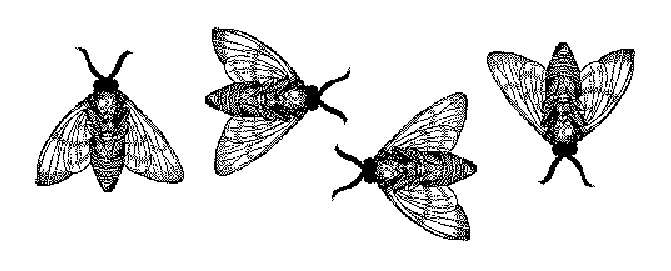
\includegraphics{flies}
\caption{A sample black and white graphic
that needs to span two columns of text.}
\end{figure*}


\begin{figure}
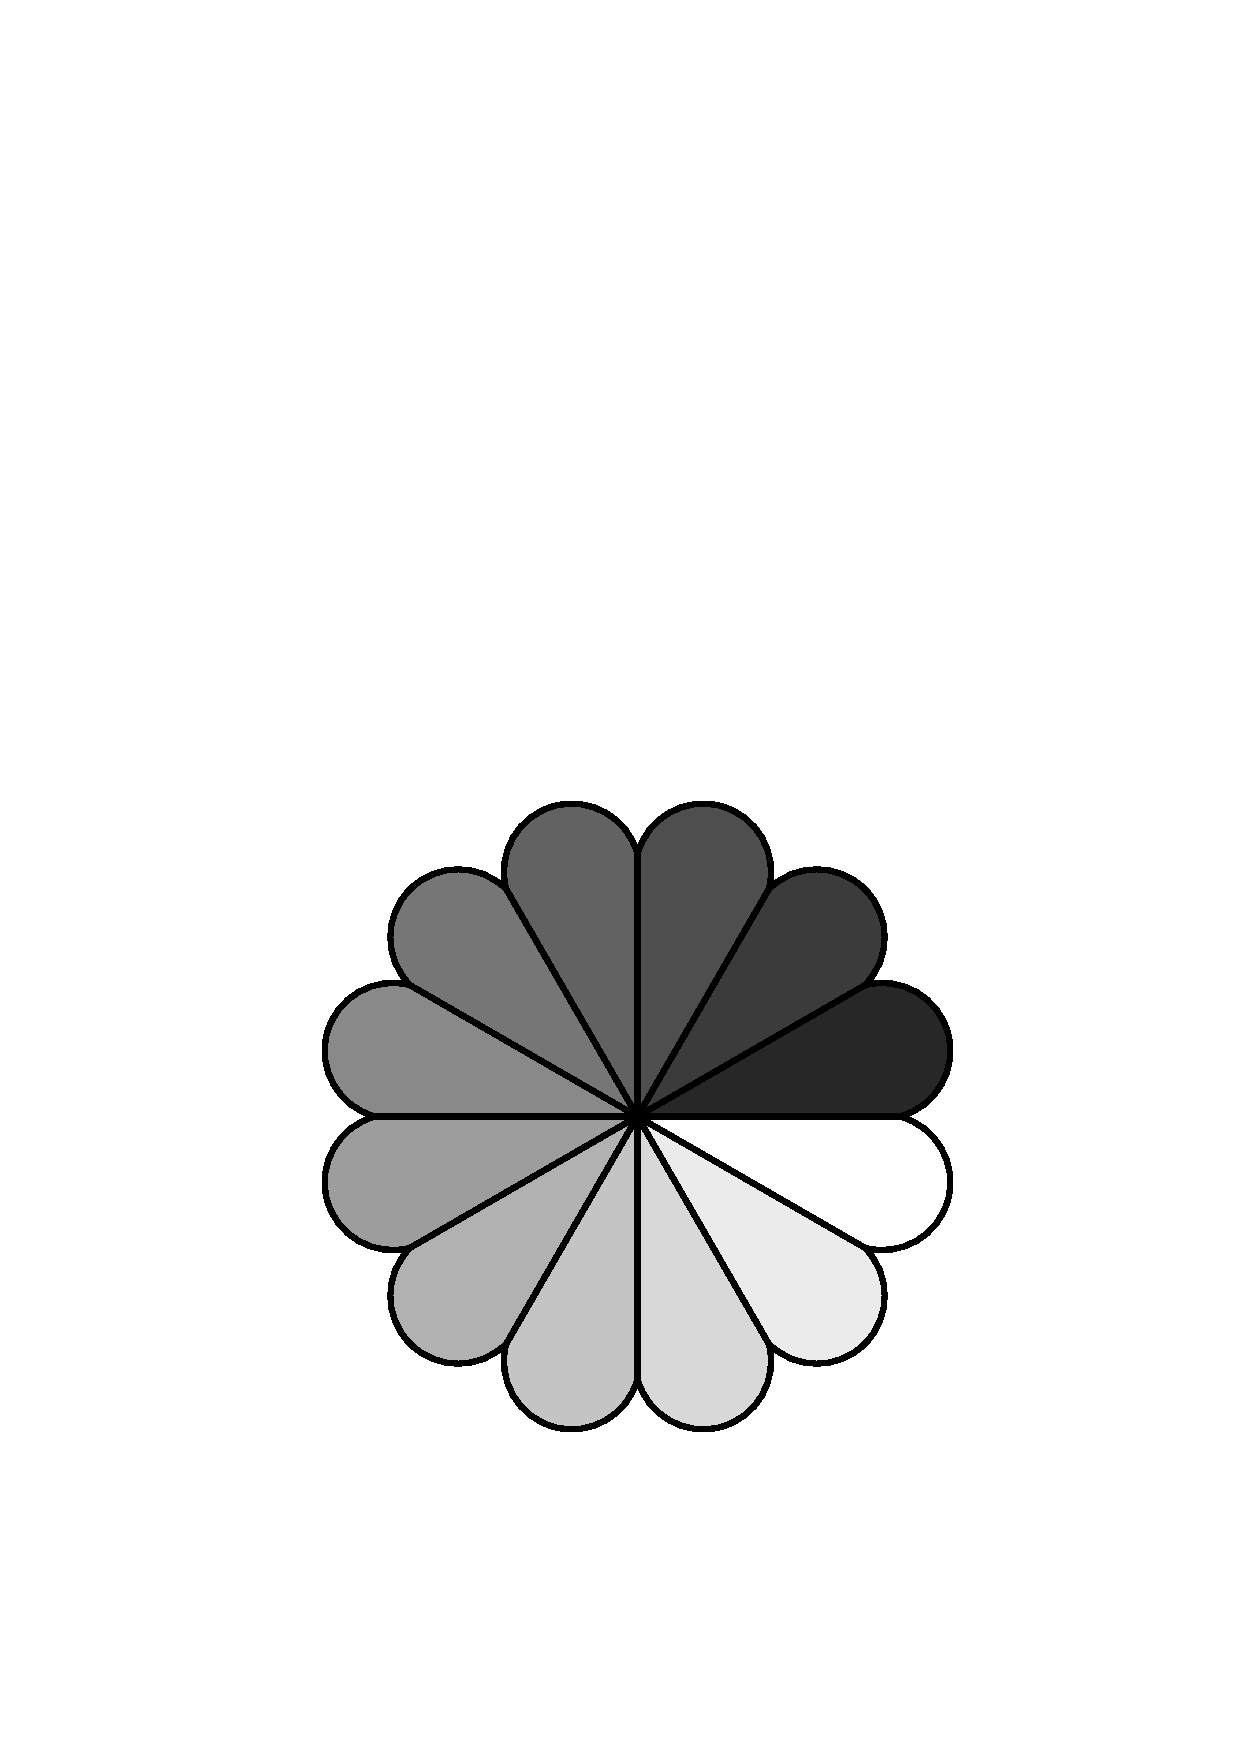
\includegraphics[height=1in, width=1in]{rosette}
\caption{A sample black and white graphic that has
been resized with the \texttt{includegraphics} command.}
\end{figure}

\subsection{Theorem-like Constructs}

Other common constructs that may occur in your article are the forms
for logical constructs like theorems, axioms, corollaries and proofs.
ACM uses two types of these constructs:  theorem-like and
definition-like.

Here is a theorem:
\begin{theorem}
  Let $f$ be continuous on $[a,b]$.  If $G$ is
  an antiderivative for $f$ on $[a,b]$, then
  \begin{displaymath}
    \int^b_af(t)\,dt = G(b) - G(a).
  \end{displaymath}
\end{theorem}

Here is a definition:
\begin{definition}
  If $z$ is irrational, then by $e^z$ we mean the
  unique number that has
  logarithm $z$:
  \begin{displaymath}
    \log e^z = z.
  \end{displaymath}
\end{definition}

The pre-defined theorem-like constructs are \textbf{theorem},
\textbf{conjecture}, \textbf{proposition}, \textbf{lemma} and
\textbf{corollary}.  The pre-defined de\-fi\-ni\-ti\-on-like constructs are
\textbf{example} and \textbf{definition}.  You can add your own
constructs using the \textsl{amsthm} interface~\cite{Amsthm15}.  The
styles used in the \verb|\theoremstyle| command are \textbf{acmplain}
and \textbf{acmdefinition}.

Another construct is \textbf{proof}, for example,

\begin{proof}
  Suppose on the contrary there exists a real number $L$ such that
  \begin{displaymath}
    \lim_{x\rightarrow\infty} \frac{f(x)}{g(x)} = L.
  \end{displaymath}
  Then
  \begin{displaymath}
    l=\lim_{x\rightarrow c} f(x)
    = \lim_{x\rightarrow c}
    \left[ g{x} \cdot \frac{f(x)}{g(x)} \right ]
    = \lim_{x\rightarrow c} g(x) \cdot \lim_{x\rightarrow c}
    \frac{f(x)}{g(x)} = 0\cdot L = 0,
  \end{displaymath}
  which contradicts our assumption that $l\neq 0$.
\end{proof}

\section{Conclusions}
This paragraph will end the body of this sample document.
Remember that you might still have Acknowledgments or
Appendices; brief samples of these
follow.  There is still the Bibliography to deal with; and
we will make a disclaimer about that here: with the exception
of the reference to the \LaTeX\ book, the citations in
this paper are to articles which have nothing to
do with the present subject and are used as
examples only.
%\end{document}  % This is where a 'short' article might terminate



\appendix
%Appendix A
\section{Headings in Appendices}
The rules about hierarchical headings discussed above for
the body of the article are different in the appendices.
In the \textbf{appendix} environment, the command
\textbf{section} is used to
indicate the start of each Appendix, with alphabetic order
designation (i.e., the first is A, the second B, etc.) and
a title (if you include one).  So, if you need
hierarchical structure
\textit{within} an Appendix, start with \textbf{subsection} as the
highest level. Here is an outline of the body of this
document in Appendix-appropriate form:
\subsection{Introduction}
\subsection{The Body of the Paper}
\subsubsection{Type Changes and  Special Characters}
\subsubsection{Math Equations}
\paragraph{Inline (In-text) Equations}
\paragraph{Display Equations}
\subsubsection{Citations}
\subsubsection{Tables}
\subsubsection{Figures}
\subsubsection{Theorem-like Constructs}
\subsubsection*{A Caveat for the \TeX\ Expert}
\subsection{Conclusions}
\subsection{References}
Generated by bibtex from your \texttt{.bib} file.  Run latex,
then bibtex, then latex twice (to resolve references)
to create the \texttt{.bbl} file.  Insert that \texttt{.bbl}
file into the \texttt{.tex} source file and comment out
the command \texttt{{\char'134}thebibliography}.
% This next section command marks the start of
% Appendix B, and does not continue the present hierarchy
\section{More Help for the Hardy}

Of course, reading the source code is always useful.  The file
\path{acmart.pdf} contains both the user guide and the commented
code.

\begin{acks}
  The authors would like to thank Dr. Yuhua Li for providing the
  MATLAB code of the \textit{BEPS} method.

  The authors would also like to thank the anonymous referees for
  their valuable comments and helpful suggestions. The work is
  supported by the \grantsponsor{GS501100001809}{National Natural
    Science Foundation of
    China}{http://dx.doi.org/10.13039/501100001809} under Grant
  No.:~\grantnum{GS501100001809}{61273304}
  and~\grantnum[http://www.nnsf.cn/youngscientists]{GS501100001809}{Young
    Scientists' Support Program}.

\end{acks}


\bibliographystyle{ACM-Reference-Format}
\bibliography{sample-bibliography}

\end{document}
